
\documentclass{beamer} 
\usetheme{Singapore}
%\usecolortheme{beaver}

\usepackage[utf8]{inputenc}
\usepackage[portuguese]{babel}
\usepackage{lmodern}
\usepackage[absolute,overlay]{textpos}
\usepackage{verbatim}
\newenvironment{reference}[2]{% 
  \begin{textblock*}{\textwidth}(#1,#2) 
      \footnotesize\it\bgroup\color{red!50!black}}{\egroup\end{textblock*}} 
\title[Ciencia y FLOSS]{Ciencia y software libre}
\author[Lopez. V.L.O]{Víctor Leonel Orozco}
\institute[UFSM]{
  Centro de Tecnologia \\
  Universidade Federal de Santa Maria
}
\date{\today}

\begin{document}
\begin{frame}[Plain]
\titlepage
\end{frame}

\begin{frame}
\frametitle{Tematica}
\tableofcontents
\end{frame}

\section{Difusión científica}
\begin{frame}{Objetivos de la difusión cientifica}
\begin{itemize}
\item Beneficiar a otros con el conocimiento
\item Obtener opiniones de otros
\item No reinventar la rueda
\item Posibilitar que otros continúen el trabajo
\end{itemize}
\end{frame}

\begin{frame}{En capitulos anteriores . . .}

\begin{figure}[tbph]
\centering
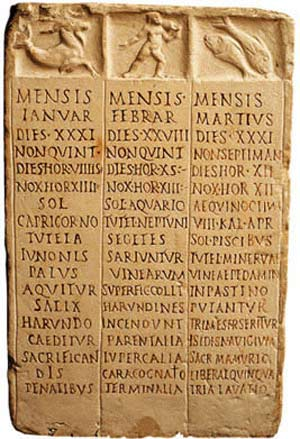
\includegraphics[width=0.35\linewidth]{Figures/1360}
\caption{Griegos}
\label{fig:1360}
\end{figure}
\end{frame}

\begin{frame}{En capitulos anteriores . . .}

\begin{figure}[tbph]
\centering
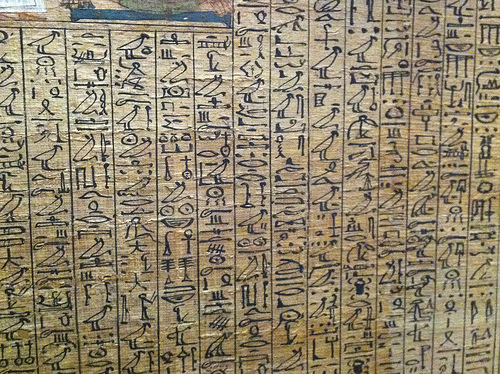
\includegraphics[width=0.7\linewidth]{./Figures/Libro-de-los-muertos}
\caption{Egipcios}
\label{fig:Libro-de-los-muertos}
\end{figure}
\end{frame}

\begin{frame}{En capitulos anteriores . . .}

\begin{figure}[tbph]
\centering
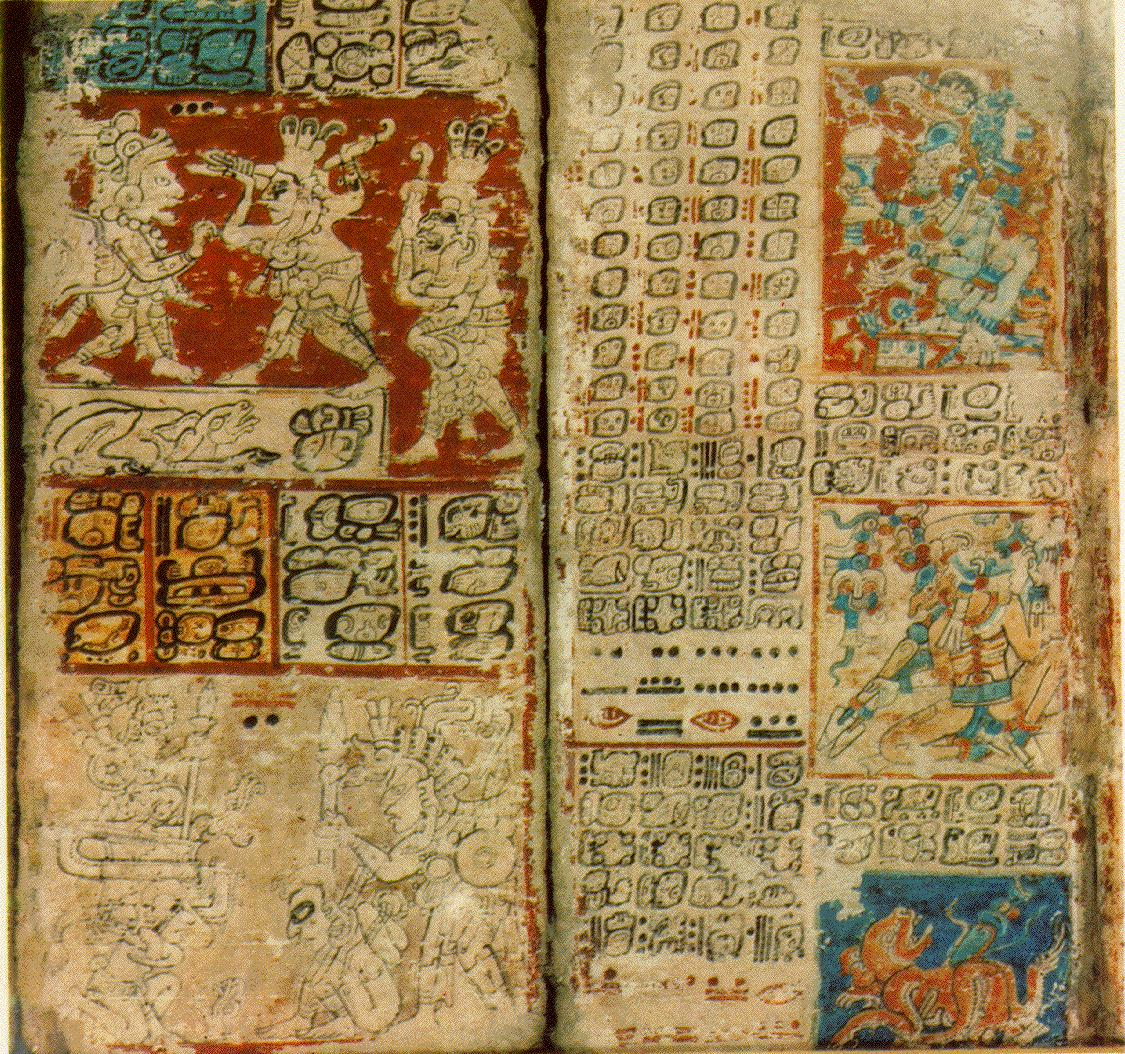
\includegraphics[width=0.50\linewidth]{./Figures/dresden}
\caption{Mayas}
\label{fig:dresden}
\end{figure}

\end{frame}

\begin{frame}{En capitulos anteriores . . .}
\begin{itemize}
\item Reservada a los eruditos/escribas/nerds de la antigüedad
\item Financiamiento aristocrático
\item Curiosidad de quien no necesitaba trabajar y/o tenia un lugar definido en la sociedad
\end{itemize}
\end{frame}

\begin{frame}{Cultura libro/paper}
\begin{itemize}
\item Los doctos necesitaban difundir lo que hacían (sigue siendo un club aristocratico)
\item Principalmente estudios religiosos que se derivaron en otras áreas de conocimiento
\item Nacen las universidades (Bolonia, Oxford, París, Módena)
\item Nacen los libros
\end{itemize}
\end{frame}

\begin{frame}{Cultura libro/paper}
\begin{itemize}
\item Modernización del conocimiento
\item Aumentan los libros
\item Desiderius Erasmus (Erasmus Mundus)
\item Nacen los papers (intros rapidas y concisas)
\item Libros: Conocimiento consolidado
\item Papers: Conocimiento de punta
\end{itemize}
\end{frame}

\begin{frame}{Cultura libro/paper}
\begin{figure}[tbph]
\centering
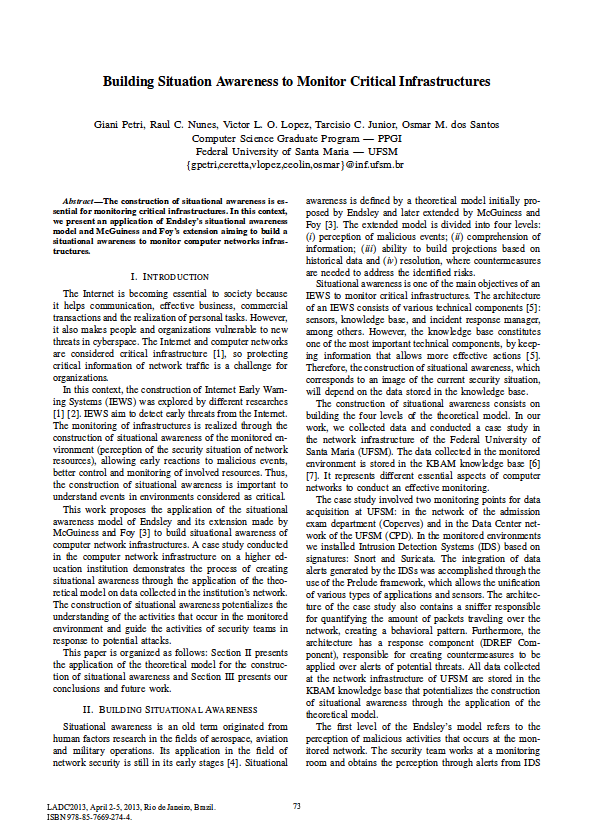
\includegraphics[width=0.7\linewidth]{Figures/Selection_001}
\caption{Paper}
\end{figure}
\end{frame}


\begin{frame}{Cultura libro/paper}
\begin{itemize}
\item Los papers se envían a revistas/congresos
\item Un comité evaluá el merito del trabajo (peer-review de PhD)
\item El paper es aceptado o rechazado
\item Es un proceso costoso y que actualmente requiere de mucho dinero (de .gt solo UFM, UVG y USAC tienen suscripciones a ciertos journals, bastante pobres)
\item Una investigación requiere de muchos papers (215)
\end{itemize}
\end{frame}

\begin{frame}{Cultura libro/paper}
\begin{figure}[tbph]
\centering
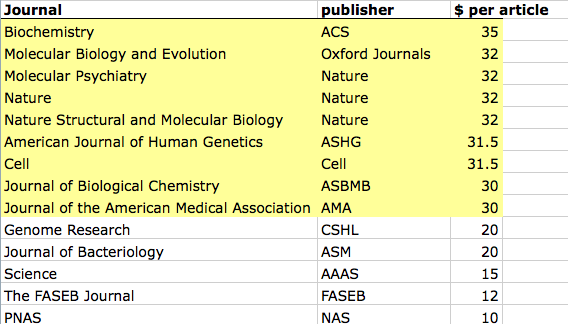
\includegraphics[width=0.65\linewidth]{./Figures/costo.png}
\caption{Costos 2012}
\label{fig:costos}
\end{figure}
\end{frame}


\begin{frame}{Cultura patente}
\begin{itemize}
\item 1421 - Felippo Brunellesch - Italia
\item 1449 - John de Utynam - Inglaterra
\item Evitar la difusión y el lucro con la idea de otro
\end{itemize}
\end{frame}

\begin{frame}{Estado 2013}
\begin{itemize}
\item Limite de acceso al conocimiento por los costos de los papers
\item Limite en general por el mal uso de las patentes
\item Difusión científica nace abierta y se convirtió en un modelo cerrado solo disponible a aquellos que tengan recursos
\item Mantener la estructura de revisión es un proceso complicado
\item En América Latina a excepción de Brasil, Chile y más recientemente México y Costa Rica la ciencia no ha despegado ni se considera importante para los gobiernos\cite{Latorre1990}
\end{itemize}



\end{frame}

\section{Cultura hacker}
\begin{frame}{Cultura hacker}
\begin{itemize}
\item La cultura hacker, nace en las ciencias exactas que desarrollan software (matemática, física, electrónica)
\item MIT
\item Los programas de computadora solían no tener valor comparado al hardware
\item Al volverse el software un negocio (he ahi el patron), se empieza a patentar y limitar el software
\item Un barbudo loco no quería imprimir y levantarse de su silla pero Xerox le limita el acceso al software
\end{itemize}
\end{frame}


\begin{frame}{Cultura hacker}
\begin{figure}[tbph]
\centering
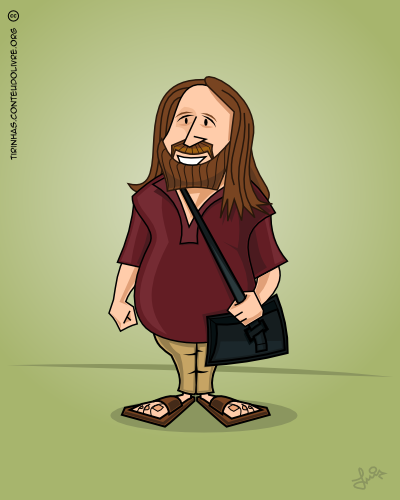
\includegraphics[width=0.7\linewidth]{Figures/Richard_Stallman_Cartoon_by_pequeno3d}
\caption{}
\label{fig:Richard_Stallman_Cartoon_by_pequeno3d}
\end{figure}
\end{frame}

\begin{frame}{Cultura hacker}
\begin{itemize}
\item Conocimiento vs. lucro
\item Innovación de capital vs. innovación colectiva
\item Un debate que aun no termina . . .
\end{itemize}
\end{frame}


\section{La nueva cultura de innovación}


\begin{frame}{FLOSS}
\begin{itemize}
\item Despego como modelo de desarrollo
\item Despego como modelo de libertad
\item Despego como modelo de negocios
\item Soporte para que la innovación continuara, dando herramientas y creando más herramientas
\end{itemize}
\end{frame}

\begin{frame}{FLOSS en ciencia y universidades}
\begin{itemize}
\item Licencias: MIT y BSD
\item Linux (Helsinki), Postgresql(U. Berkley - Ingres), LLVM (U. Illinois Urbana-Champaign), HTTP (CERN), Darwin (Carnegie Mellon - Match), Tex (Stanford), Beowulf (NASA), Lua (PUC-Rio)
\item En general el software libre facilita la investigación
\end{itemize}
\end{frame}

\begin{frame}{Influencia en la ciencia}
\begin{itemize}
\item El hijo prodigo regresa a dar lecciones
\item Open access
\item Creative commons
\end{itemize}
\end{frame}

\begin{frame}{Open access}
\begin{itemize}
\item Acceso libre a las investigaciones científicas
\item Europa
\item Traslada el costo de revisión de papers al que quiere publicar :(
\end{itemize}
\begin{figure}[tbph]
\centering

\includegraphics[width=0.25\linewidth]{Figures/Open_Access_logo.png}
\caption{Open Access}
\label{fig:open}
\end{figure}
\end{frame}

\begin{frame}{Creative commons}
\begin{itemize}
\item Licencia ampliamente aceptada en trabajos independientes (arte, dorumentación, wikipedia)
\item Revista nature ya permite elegir creative commons \cite{Nature}
\end{itemize}
\begin{figure}[tbph]
\centering

\includegraphics[width=0.25\linewidth]{Figures/creative-commons-logo-640-80.jpg}
\caption{Creative commons}
\label{fig:cc}
\end{figure}
\end{frame}

\begin{frame}{Estado actual}
\begin{itemize}
\item Ambos modelos de innovación coexisten compitiendo entre si \cite{Drive2003}
\item Los modelos de innovación abierta están siendo ampliamente aceptados en todas partes del mundo, Europa \cite{Europa2013}, USA \cite{USA2013} y a nuestro nivel en Mexico\cite{Mx2013} y Brasil\cite{Br2013-}
\item Muchas de las personas que contribuyen en Software Libre han sido pioneros en la creación de nuevas ideas y practicas acerca de licenciamiento y propiedad intelectual en los procesos de innovación \cite{VonKrogh2006}
\end{itemize}
\end{frame}

\section{Consideraciones finales}
\begin{frame}{Consideraciones finales}
\begin{itemize}
\item Actualmente mucha de la ciencia es soportada por software libre o esta generando software libre
\item La ciencia jugo un papel fundamental para inspirar la creación de software libre tanto por necesidades tecnológicas, como para acceso al conocimiento
\item El software libre encontró el punto para coexistir donde la ciencia aun esta trabajando (merito cientifico vs. meritocracia por difusión)
\item Países como el nuestro tienen una gran oportunidad porque los sistemas académicos ni siquiera existen y no hay que enfrentar resistencia al cambio
\item Ademas el acceso abierto mejoraría nuestro acceso al conocimiento
\end{itemize}
\end{frame}


\begin{frame}{Contacto}
\begin{itemize}
\item http://tuxtor.shekalug.org
\item tuxtor@shekalug.org
\item http://github.com/tuxtor/slides
\end{itemize}
\begin{center}

\includegraphics[width=0.1\linewidth]{Figures/cclogo}
\\
This work is licensed under a Creative Commons Attribution-ShareAlike 3.0 Brazil License.
\end{center}
\end{frame}

\section{Referencias}
\begin{frame}[allowframebreaks]{Referencias}
    \bibliographystyle{IEEEtran}
    \bibliography{refs}
\end{frame}
\end{document}